\begin{figure}[htbp]
\centering
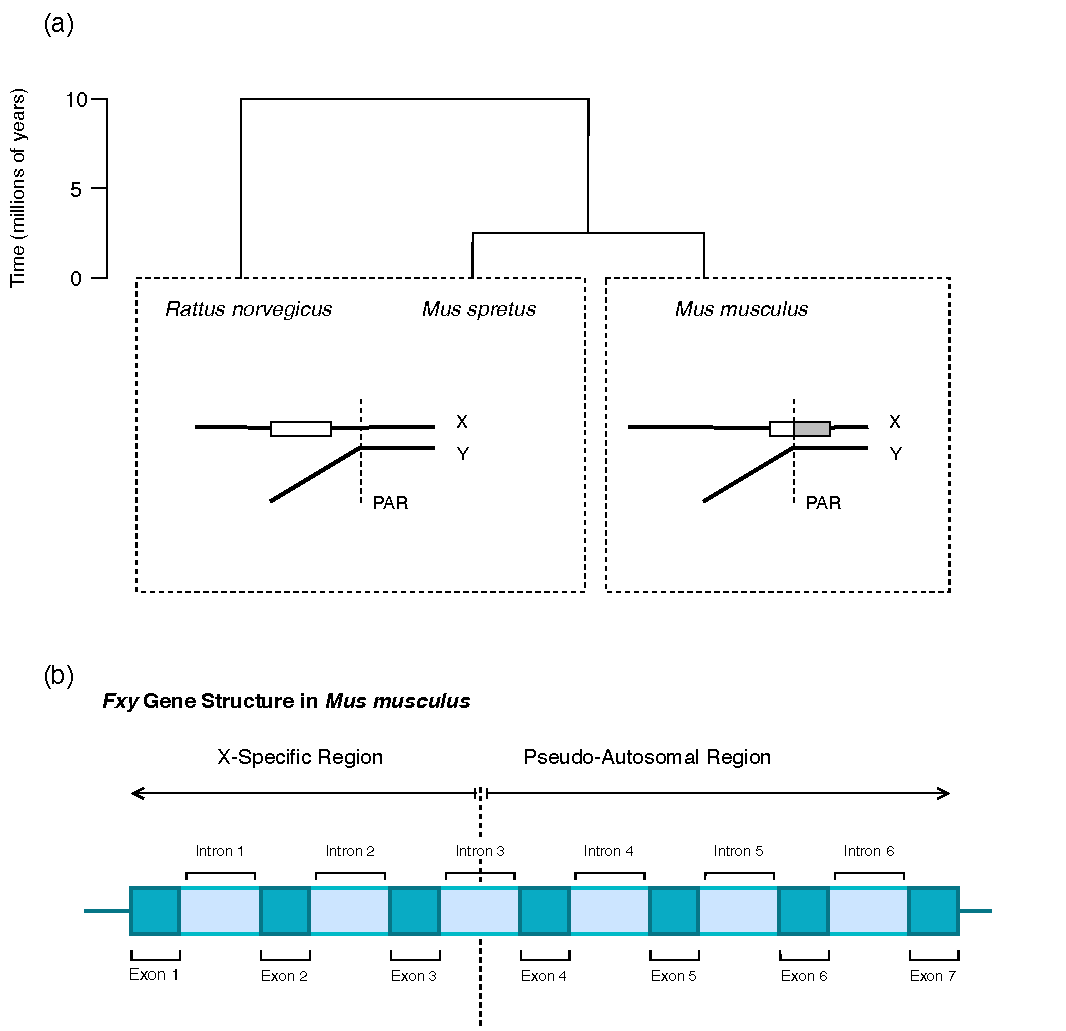
\includegraphics[width=\textwidth]{figures/diagrams/Fxy.pdf}
\caption{\textbf{Evolutionary History of \textit{Fxy} in Rodents}. \textbf{(a)} The \textit{Fxy} gene in \textit{M. musculus} was translocated from a X-linked position to a new position in which it overlaps with the PAR. The overlap in \textit{M. musculus} is shown as the shaded region of the gene, shown as a box. In other rodents, including \textit{M. spretus} and \textit{R. } The phylogeny in (a) is adapted from Figure 1 in \cite{Galtier2007AdaptationEvolution}}
\label{fig:Fxy}
\end{figure}